\section{Cumulative cost curve}

The cumulative cost curve shows the added costs of the project along its duration. The following graph has been done taking into account the daily salary of the workers as well as the daily cost of the facilities. Two main steps can be appreciated which represents the investment in hardware in order to do the prototypes and the validations. Moreover, notice that by day 1 the costs are of around 42000\euro, which represent the initial expenses to pay the software of the project.

%\begin{figure}[H]
%	\centering
%	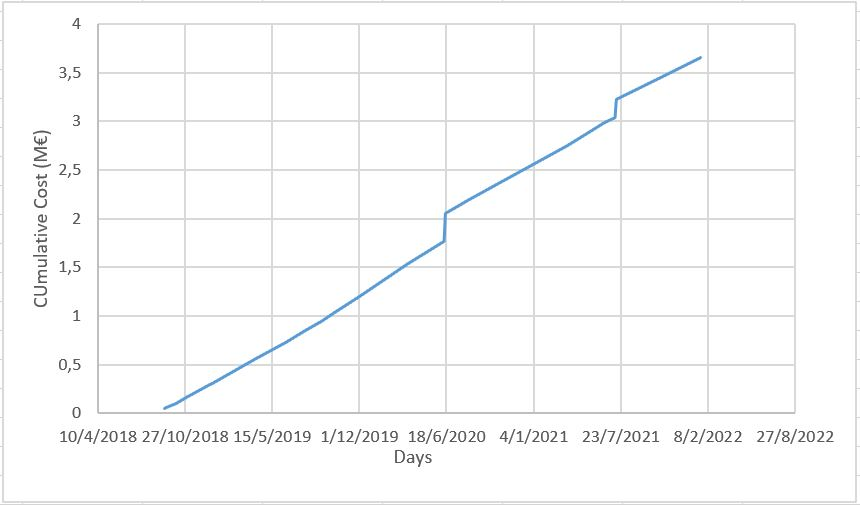
\includegraphics[width=0.65\linewidth]{./images/CumulativeCost}
%	\caption[Cumulative Cost Curve over time]{Cumulative Cost Curve over time \cite{workfront2017}.}
%	\label{fig:CumulativeCost}
%\end{figure} 

\begin{figure}[H]
	\centering
	\begin{tabular}{@{}c@{\hspace{.5cm}}c@{}}
		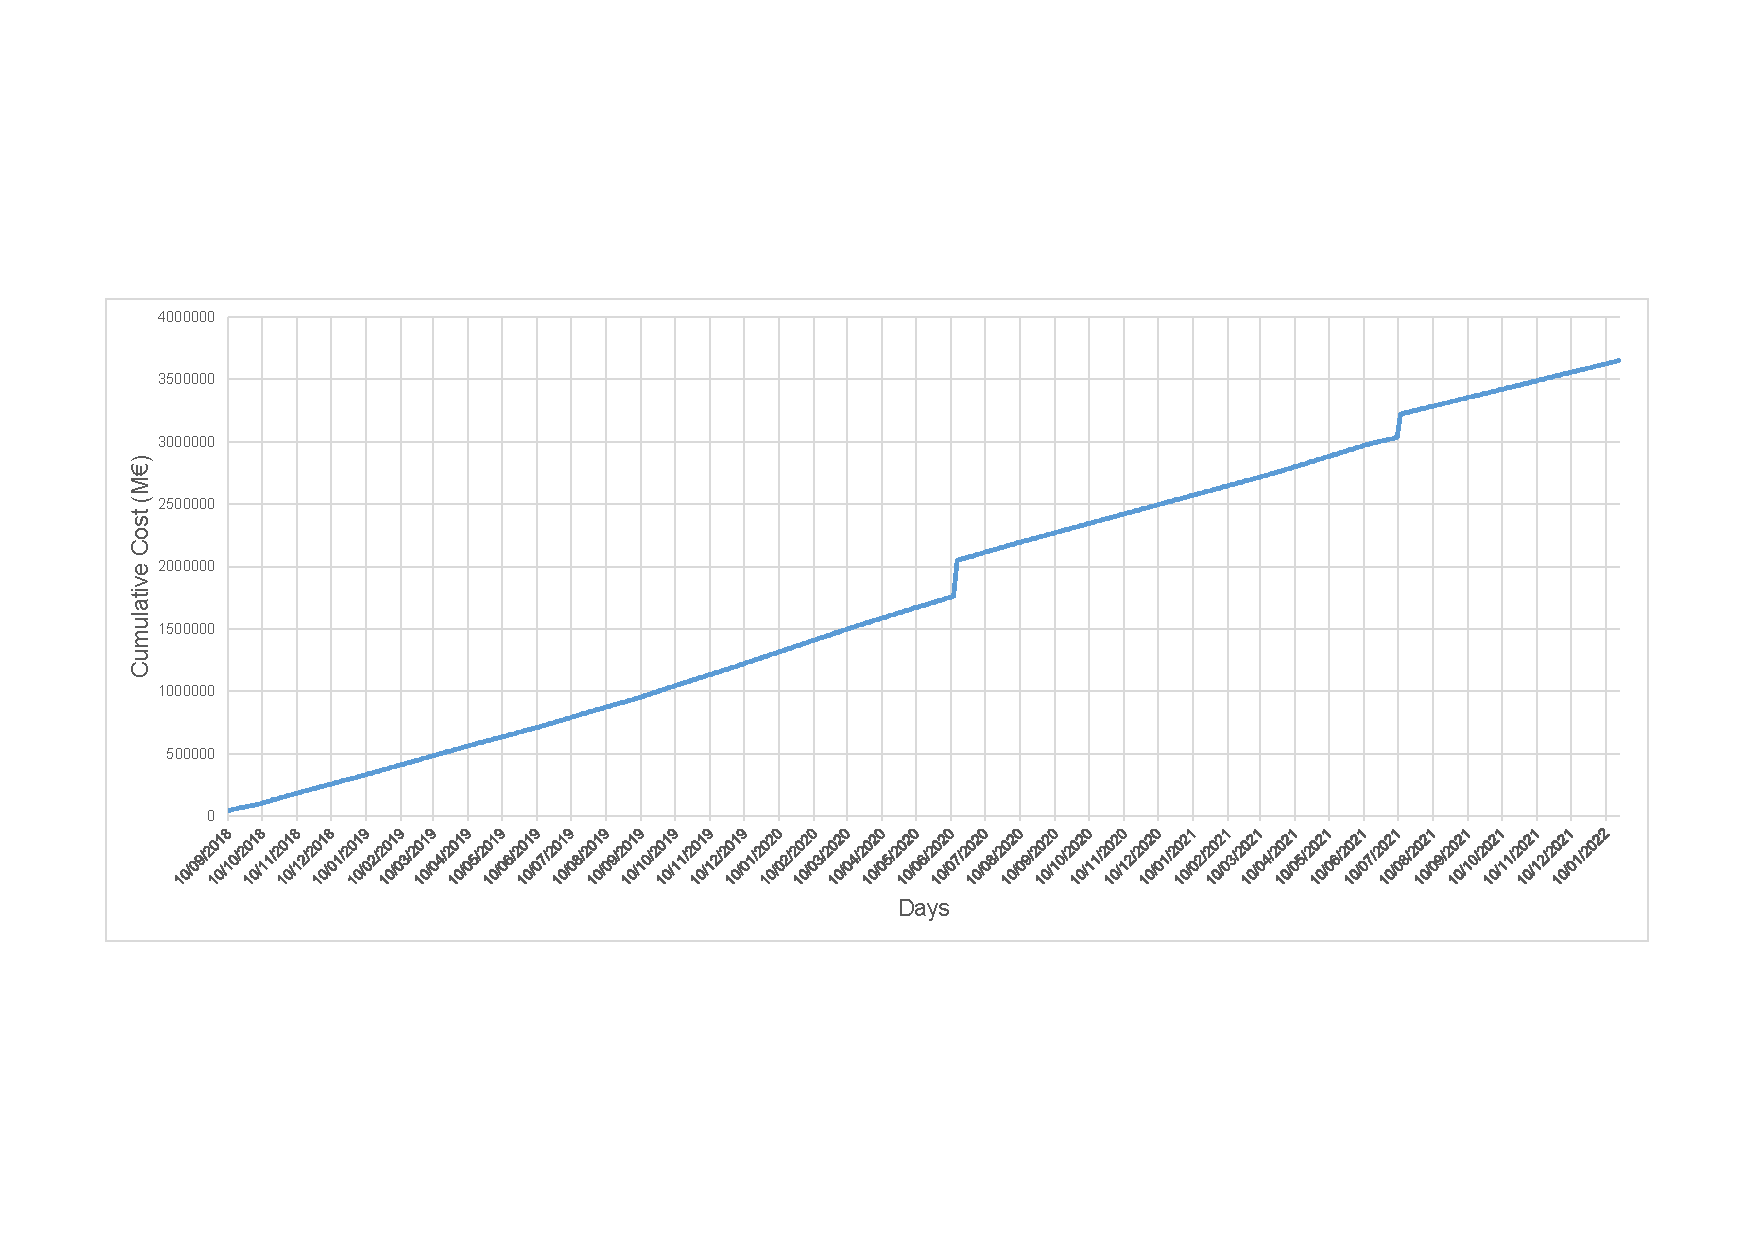
\includegraphics[page=1,width=1\textwidth, trim={2cm 5.2cm 2cm 5.2cm},clip]{./images/CumulativeCost.pdf}
	\end{tabular}
	\caption{Cumulative Cost Curve over time \cite{workfront2017}.}
	\label{fig:CumulativeCost}
\end{figure}

The information that this curve gives is crucial in order to be able to schedule the project cash flow. Indeed, it is a perfect reference to avoid budget overrun along the follow up of the project. Finally, budget at completion, as indicated before is estimated to be around \textbf{3.65M\euro}.